%%
%% main.tex - Memoria de la tesis
%%
%%   Copyright 2009-2010 Jesús Torres <jmtorres@ull.es>
%%
%% Esta obra está bajo licencia Creative Commons Reconocimiento 3.0 Unported
%%
\documentclass[b5paper,twoside,11pt,DIV=calc]{scrbook}
\KOMAoptions{open=right,cleardoublepage=empty,headings=big,headsepline=true,
  chapterprefix,bibliography=totoc,captions=tableheading,numbers=enddot,
  draft=false}
\addtocounter{tocdepth}{-1} % No mostrar las subsecciones en las TOC

% Idioma
% http://www.tex-tipografia.com/spanish2.html
% \usepackage[spanish,es-noenumerate,es-tabla]{babel}
\usepackage[british,UKenglish,USenglish,english,american]{babel}
\selectlanguage{english}
\usepackage{ucs}
\usepackage[utf8x]{inputenc}
\usepackage[T1]{fontenc}

\usepackage{float}

% \renewcommand*{\USenglishcontentsname}{\'Indice}

% Fuentes
\usepackage{mathpazo} % Texto con "Palatino" + fuente matemática "Pazo"
\renewcommand{\sfdefault}{uop} % "Optima" como fuente sans serif
\setkomafont{pagehead}{\sffamily\small}
\setkomafont{pagenumber}{\usekomafont{pagehead}}
\setkomafont{caption}{\sffamily\small}
\addtokomafont{captionlabel}{\bfseries}

% Interlineado
\usepackage{setspace}
\onehalfspacing

\recalctypearea % Recalcular las áreas de los bloques de texto
% \usepackage[a4,center,frame]{crop} % Marcas de corte
% \usepackage{showframe} % Marcar los márgenes

% Espacio anterior y posterior al título de cada capítulo
\renewcommand*{\chapterheadstartvskip}{\vspace*{4.50\baselineskip}}
\addtokomafont{chapter}{\fontsize{26}{26}\selectfont}
%\renewcommand*{\chapterheadendvskip}{\vspace{2.25\baselineskip}}

% Listas
% \spanishsignitems

% Notas al pié
\usepackage[multiple]{footmisc}
\deffootnote{1.25em}{1.75em}{\textsuperscript{\thefootnotemark}}

% Separador del título de figuras y tablas
\renewcommand*{\figureformat}{\figurename~\thefigure}
\renewcommand*{\tableformat}{\tablename~\thetable}
\renewcommand*{\captionformat}{\autodot\enskip}
\setcapindent{0em}

% Subfiguras
\usepackage[caption=false, % Usar los captions de KOMA-script
            labelformat=simple]{subfig}
\renewcommand\thesubfigure{(\alph{subfigure})} % Paréntesis en las subfiguras
\renewcommand\thesubtable{(\alph{subtable})} % Paréntesis en las subtablas

% Tablas
\usepackage{longtable} % notación
\usepackage{tabularx}
\usepackage{booktabs}
\newcolumntype{C}{>{$}c<{$}}
\newcolumntype{L}{>{$}l<{$}}
\newcolumntype{R}{>{$}r<{$}}
\renewcommand*{\arraystretch}{1.1} % Distancia entre filas

% Comando para ayudar a formatear los nombres de los programas
\usepackage{xspace}
\newcommand*{\program}[1]{{\ttfamily #1}}
\newcommand{\Blender}{\program{Blender}\xspace}
\newcommand{\Matlab}{\program{MATLAB}\xspace}
\newcommand{\Makehuman}{\program{MakeHuman}\xspace}

% Listados de código
\usepackage{listings}
\lstset{basicstyle=\small}
\newcommand*{\lstCppMakeShortInline}[1]
  {\lstMakeShortInline[language=C++,basicstyle=\normalsize\ttfamily]#1}
\newcommand*{\lstMatlabMakeShortInline}[1]
  {\lstMakeShortInline[language=MATLAB,basicstyle=\normalsize\ttfamily]#1}
\newcommand*{\lstPythonMakeShortInline}[1]
  {\lstMakeShortInline[language=Python,basicstyle=\normalsize\ttfamily]#1}

% Algoritmos
\usepackage{algorithmic}
\usepackage{algorithm}

% Gráficos
\usepackage{tikz}
\usepackage{graphicx}
\newlength{\figuresheight}
\setlength{\figuresheight}{7cm}
\setkeys{Gin}{totalheight=\figuresheight,keepaspectratio=true}
\graphicspath{{./images/bmps/}{./images/vects/}{./images/}}
\usepackage{ifpdf}
\ifpdf
  \DeclareGraphicsExtensions{.pdf,.mps,.png,.jpg}
\else
  \DeclareGraphicsExtensions{.eps,.mps}
\fi

% Bibliografía
% Citas ordenadas en el orden en que aparecen en la bibliografía (sort).
% % En la primera cita aparecen los nombres de todos los autores (longnamesfirst)
% % \usepackage[longnamesfirst,sort]{natbib}
\usepackage[sort]{natbib}
\bibliographystyle{abbrvnat}
\bibpunct{(}{)}{;}{a}{,}{,}
\setbibpreamble{Las siguientes referencias bibliográficas se presentan en orden
alfabético por autor. Las referencias con más de un autor aparecen ordenadas
en base al primero de los mismos.\par\bigskip}

% Referencias
\usepackage[spanish]{varioref}
\labelformat{enumi}{(#1)}
\labelformat{equation}{(#1)}

% PDFTeX
\pdfimageresolution=300
\pdfcompresslevel=9
\pdfadjustspacing=1 % Asegurar la compatibilidad con la salida normal de TeX
\usepackage[
  bookmarksnumbered=true,
  pdfborder={0 0 0},
  pdfdisplaydoctitle=true,
  pdftitle={T\'itulo de la tesis},
  pdfauthor={Autor de la tesis},
  pdfsubject={Memoria de tesis doctoral},
  pdfkeywords={memoria, tesis, plantilla, latex}
  ]{hyperref}

% Para las páginas apaisadas
% \usepackage{lscape}
% \usepackage{pdflscape}
\usepackage{rotfloat} % TODO: Páginas apaisadas en el PDF

% Matemáticas
\usepackage{amsmath}
% \unaccentedoperators
\newcommand{\relphantom}[1]{\mathrel{\phantom{#1}}}
\newcommand{\func}[1]{\mathnormal{#1}}
\newcommand{\mat}[1]{\boldsymbol{\mathrm{\MakeUppercase{#1}}}}
\newcommand{\spc}[1]{\mathbb{#1}}
\newcommand{\dist}[1]{\mathcal{#1}}
\renewcommand{\vec}[1]{\boldsymbol{#1}}
\newcommand{\UPSIGMA}{\boldsymbol{\Sigma}}

\usepackage[printonlyused,withpage]{acronym}
\usepackage{local}

% Estructura del documento
\begin{document}

\frontmatter
\label{portada}\pdfbookmark{Tesis doctoral}{portada}
\titlehead{\includegraphics[height=1cm]{unilogo} \\
  \vskip 1em
  Centro de la Universidad \\
  Departamento de la Universidad}
\subject{Tesis doctoral}
\title{Título de la tesis}
\author{Autor de la tesis}
\date{2010}
\maketitle

%%
%% certificado.tex - Memoria de la tesis
%%
%%   Copyright 2009-2010 Jesús Torres <jmtorres@ull.es>
%%
%% Esta obra está bajo licencia Creative Commons Reconocimiento 3.0 Unported
%%
\cleardoublepage
\thispagestyle{empty}
\hfill\begin{minipage}[t]{0.85\textwidth}\parindent 3em
D. DIRECTOR DE LA TESIS, Doctor en TITULACIÓN y CATEGORÍA DEL DIRECTOR de
DEPARTAMENTO DEL DIRECTOR DE LA TESIS de la UNIVERSIDAD DEL DIRECTOR.
\null\vspace{\baselineskip}
CERTIFICA:

\vspace{\baselineskip}
que D. DOCTORANDO, TITULO DEL DOCTORANDO, ha realizado bajo mi
dirección la presente Tesis, titulada ``TÍTULO DE LA TESIS'', para optar al
grado de Doctor por la UNIVERSIDAD QUE CORRESPONDA.

\vspace{\baselineskip}
Con esta fecha, autorizo la presentación de la misma.

\vspace{\baselineskip}
\hfill En LUGAR, a FECHA.
\end{minipage}

\vspace{\baselineskip}
\hfill\begin{tabular}{c}
El Director, \\\\\\\\
DIRECTOR DE LA TESIS
\end{tabular}

%%
%% dedicatoria.tex - Memoria de la tesis
%%
%%   Copyright 2009-2010 Jesús Torres <jmtorres@ull.es>
%%
%% Esta obra está bajo licencia Creative Commons Reconocimiento 3.0 Unported
%%
\cleardoublepage
\thispagestyle{empty}
\null\vskip 1cm
\textit{\raggedleft
  A Uchy.\\
  \vskip 4cm
  A mis padres, Bernardo e Inmaculada,\\*
  y a mi hermana, Esther.\\
}

%%
%% agradecimientos.tex - Memoria de la tesis
%%
%%   Copyright 2009-2010 Jesús Torres <jmtorres@ull.es>
%%
%% Esta obra está bajo licencia Creative Commons Reconocimiento 3.0 Unported
%%
\cleardoublepage
\thispagestyle{empty}
\addsec*{\protect\centering Agradecimientos}
\markboth{Agradecimientos}{}

En primer lugar, me gustaría agradecer a mis directores de Tesis, Dr. D. Leopoldo Acosta Sánchez y Dr. D. Jonay Tomás Toledo Carrillo, la oportunidad de colaborar en este proyecto, sin el cual no podría haber aprendido lo que he aprendido, ver lo que visto, ni hacer lo que entre todos hemos hecho. Y por supuesto, los buenos consejos y el tiempo prestado, que no ha sido poco, especialmente en las últimas semanas de la Tesis.

No puedo quedarme sin dar mi agradecimiento al Dr. D. Jesús Javier Espelosín Ortega, D. Rafael Arnay del Arco y D. Daniel Perea Ström (¡equipo MARANEDA!), y D. Jonatán Felipe, con los que empecé este camino de cabras que parece no terminar nunca. Nadie nos contó que estaba sin asfaltar, pero estuvimos lo suficientemente locos como para seguir. Agradezco el apoyo ofrecido todos estos años, y sobre todo el buen humor, que nunca ha faltado. Igualmente, agradezco al Dr. D. Jesús Miguel Torres Jorge el haber malgastado parte de su valioso tiempo resolviéndome infinitas dudas sobre todo lo que no era capaz de echar a andar por mi cuenta. 

Cómo no, al ``equipo cafeína'', por haber llevado la procastinación a niveles desconocidos. Ellos son: Dña Ángela Hernández López, D. Antonio Morell González, D. Ayoze Marrero Ramos, Dña. Elena Santos Hernández, D. Esteban Rodríguez, D. Eusebio Morell González, D. Francisco Fumero Batista, Dr. D. Iván Castilla Rodríguez, D. Javier Hernández Aceituno, Dr. D. Juan Albino Méndez Pérez (a.k.a. Alexis), Dña. Mariana Cairós González, D. Pedro Antonio Toledo Delgado, Dña. Sara González Pérez, Dña. Silvia de León, Dña. Silvia Vera González, D. Yeray Callero de León y Dña. Kelin Victoria Zúñiga Meneses. No me olvido de los infiltrados: Esther Amador, Adal Hancock, Zeus Ruiz, Elisa Sosa Trujillo, Anelia Stoyanova y Miguel Torres. Igualmente, al resto del ya extinto Departamento de Ingeniería de Sistemas y Automática y Arquitectura y Tecnología de Computadores (ISAATC): Dra. Dña. Silvia Alayón Miranda, Dra. Dña. Rosa María Aguilar Chinea, D. Ginés Coll Barbuzano, Dr. D. José Ignacio Estévez Damas, Dra. Dña. Carina Soledad González González, Dr. D. Evelio José González González, D. Germán Carlos González Rodríguez, Dr. D. Alberto Francisco Hamilton Castro, Dr. D. Sergio Elías Hernández Alonso, D. Eladio Hernández Díaz, Dr. D. Graciliano Nicolás Marichal Plasencia, Dr. D. Roberto Luis Marichal Plasencia, D. Juan Julián Merino Rubio, Dr. D. Lorenzo Moreno Ruiz, Dra. Dña. Vanesa Muñoz Cruz, Dr. D. Sid Ahmed Ould Sidha, Dr. D. José Demetrio Piñeiro Vera, D. Héctor Javier Reboso Morales, Dr. D. José Luis Sánchez de la Rosa, Dr. D. José Francisco Sigut Saavedra y Dra. Dña. Marta Sigut Saavedra.

Vorrei ringraziare il Proffesore Sig. Alberto Broggi per l'opportunità di collaborare e imparare in VisLab, e anche Dott. Paolo Zani e Dott. Mirko Felisa per aver accettato di rivedere questa noiosa tesi e il suo incondizionato supporto durante il mio soggiorno a Parma. Inoltre, apprezzo il consiglio e la grande ospitalità dimostrata da Dott. Luca Bombini, Sig. Michele Buzzoni, Sig. Gabriele Camellini, Dott. Pietro Cerri, Sig. Alessandro Coati, Dott. Rean Isabella Fedriga, Sig. Alessandro Giacomazzo, Dott. Paolo Grisleri, Dott. Paolo Medici, Dott. Pier Paolo Porta, Sig. Mario Sabbatelli e Sig. Pietro Versari, che mi hanno fatto sentire a casa. Anche Sig. Moisés Díaz Cabrera, per la compagnia.

I also want to thank Prof. Luc Van Gool for allowing me staying some months in PSI/VISICS, acquiring the expertise of his group. I want also to thank the help and the good mood of Mr. Roeland De Geest, Mr. Bert Deknuydt, Mr. Vincent De Smet, Mr. Basura Fernando, Mrs. Rosalia Galiazzi Schneider, Mr. Stam Georgoulis, Mr. Amir Ghodrati, Dr. Hakan Bilen, Mr. Xu Jia, Mr. Jan Knopp, Mr. Paul Konijn, Dr. Marco Pedersoli, Dr. Markus Mathias, Mr. Andelo Martinovic, Mr. Wim Moreau, Mr. José Antonio Oramas Mogrovejo, Mr. Konstantinos Rematas, Mr. Gilad Sharir, Dr. Radu Timofte, Dr. David Tingdahl and Dr. Tatiana Tommasi.

He dejado para el final a los que siempre han estado ahí. A Emilio Brito López, por haberme cuidado la piedra y haberme ayudado a encontrar el océano; a Beatriz Santos Hernández, por demostrar que 360 no es divisible por 5; y a Miguel Ángel Yonte Rodríguez, por recordarme que vivimos bajo la amenaza constante de que un asterisco nos caiga sobre la cabeza. No me olvido de Lilia Ana Ramos y sus consejos sobre los efectos secundarios de la amapola, Jessica Luis López y su inapropiada afición al surf carnavalero, o Ettore Gendusa, sin cuya colaboración esta sección de agradecimientos podría haber acabado en desastre. De Zebenzui Álvarez Lugo aprendí a encontrarle el punto a las cosas, y junto a Jorge Martín Afonso busqué todo lo negro.

Un reconocimiento especial a mi familia, quienes siempre han estado ahí apoyándome, animándome y, sobre todo, educándome. No puedo ignorar el hecho de que si no fuera por ellos, no podría haber llegado a lo que he llegado, ni podría haber disfrutado de ciertos privilegios de los que me siento muy agradecido. De mi madre, 
Inmaculada Hernández Gil, heredé el gusto por viajar, descubrir nuevos horizontes y llegar siempre un poco más lejos; de mi padre, Bernardo Morales Trujillo, aprendí el gusto por conocer, por aprender y por hacer bien las cosas. Este reconocimiento también va para mi hermana, Esther Morales Hernández, que aunque haya puesto mar de por medio, siempre será mi experta en series y cultura contemporánea favorita.

El último agradecimiento lo he reservado para la Doctora Esther Sanromá Ramos (Uchy para los amigos), la persona más importante en mi vida, y con la que más me alegro de haberme cruzado. Agradezco sus esfuerzos por convertirme en una persona socialmente aceptable, la tolerancia demostrada ante mis contínuos \emph{festivales del humor} y su paciencia a la hora de hacerme ver diversos errores de cálculo espaciales (1.35\,m y 1.50\,m no son lo mismo), temporales (10 minutos y media hora no son medidas equivalentes) y espectrales (aunque los árboles sean así, el marrón y el verde no combinan). Pero sobre todo, agradezco los buenos momentos y la felicidad que ha sido capaz de darme.










\cleardoublepage
\pdfbookmark{\contentsname}{tableofcontents}
\tableofcontents

\cleardoublepage
\pdfbookmark{\listtablename}{listoftables}
\listoftables

\cleardoublepage
\pdfbookmark{\listfigurename}{listoffigures}
\listoffigures

\cleardoublepage
\pdfbookmark{\listalgorithmname}{listofalgorithms}
\listofalgorithms

%%
%%  acronyms.tex - Obstacle Detection and Planning for Autonomous Vehicles based on Computer Vision Techniques
%%
%%  Copyright 2014 Néstor Morales <nestor@isaatc.ull.es>
%% 
%%  Original version: Copyright 2009-2010 Jesús Torres <jmtorres@ull.es>
%%
%%  This work is licensed under a Creative Commons Attribution 4.0 International License.

\cleardoublepage
\chapter*{Acronyms}\label{ch:acronyms}
\pdfbookmark{Acronyms}{acronyms}
\begin{acronym}[acronyms]
  \acro{RNDF}{Road Network Definition File}
  \acro{MSVM}{Multi-class Support Vector Machine}
  \acro{SVM}{Support Vector Machine}
  \acro{LIDAR}{Light-Detection And Ranging}
  \acro{HMI}{Human-Machine Interface}
  \acro{GPU}{Graphical Processing Unit}
  \acro{GPS}{Global Positioning System}
  \acro{IMU}{Inertial Measurement Unit} 
  \acro{PF}{Particle Filter}
  \acro{LGT}{Lidar Ground Truth}
  \acro{ROI}{Region of Interest}
  \acro{RRT}{Rapidly-exploring Random Trees}
  \acro{SAD}{Sum of Absolute Differences}
  \acro{DP}{Dynamic Programming}
  \acro{ELAS}{Efficient Large-Scale Stereo Matching}
  \acro{SGM}{Semi-Global Matching}
  \acro{ADAS}{Advanced Driver Assistance Systems}
  \acro{CRF}{Conditional Random Field}
  \acro{TPS}{Thin Plate Splines}
  \acro{WM}{Weighted Mean}
  \acro{PL}{Piecewise Linear}
  \acro{PCA}{Principal Component Analysis}
  \acro{ACO}{Ant Colony Optimization}
\end{acronym}

\acrodef{RNDF}[RNDF]{Road Network Definition File}
\acrodef{MSVM}[MSVM]{Multi-class Support Vector Machine}
\acrodef{SVM}[SVM]{Support Vector Machine}
\acrodef{LIDAR}[LIDAR]{Light-Detection And Ranging}
\acrodef{HMI}[HMI]{Human-Machine Interface}
\acrodef{GPU}[GPU]{Graphical Processing Unit}
\acrodef{GPS}[GPS]{Global Positioning System}
\acrodef{IMU}[IMU]{Inertial Measurement Unit}
\acrodef{PF}[PF]{Particle Filter}
\acrodef{LGT}[LGT]{Lidar Ground Truth}
\acrodef{ROI}[ROI]{Region of Interest}
\acrodef{RRT}[RRT]{Rapidly-exploring Random Trees}
\acrodef{SAD}[SAD]{Sum of Absolute Differences}
\acrodef{DP}[DP]{Dynamic Programming}
\acrodef{ELAS}[ELAS]{Efficient Large-Scale Stereo Matching}
\acrodef{SGM}[SGM]{Semi-Global Matching}
\acrodef{ADAS}[ADAS]{Advanced Driver Assistance Systems}
\acrodef{CRF}[CRF]{Conditional Random Field}
\acrodef{TPS}[TPS]{Thin Plate Splines}
\acrodef{WM}[WM]{Weighted Mean}
\acrodef{PL}[PL]{Piecewise Linear}
\acrodef{PCA}[PCA]{Principal Component Analysis}
\acrodef{ACO}[ACO]{Ant Colony Optimization}


%%
%% notacion.tex - Memoria de la tesis
%%
%%   Copyright 2009-2010 Jesús Torres <jmtorres@ull.es>
%%
%% Esta obra está bajo licencia Creative Commons Reconocimiento 3.0 Unported
%%
\chapter*{Símbolos y notación}\label{notación}
\pdfbookmark{Símbolos y notación}{notación}
\markboth{Símbolos y notación}{}
\begin{longtable}{rp{0.8\textwidth}}
  $a$               & escalar \\
  $|a|$             & valor absoluto de $a$ \\
  $\vec{a}$         & vector columna \\
  $a_i$             & $i$-ésimo elemento del vector $\vec{a}$ o del conjunto
    de escalares $\{a_n\}$  \\
  $\vec{1}$         & vector columna $[1,1,\ldots,1]^T$ \\
  $\|\vec{a}\|$     & norma euclídea de $\vec{a}$  \\
  $\vec{a}^T$       & traspuesta de $\vec{a}$ \\
  $\mat{A}$         & matriz  \\
  $\vec{a}_i$       & $i$-ésimo elemento de conjunto de vectores $\{\vec{a}_n\}$
    o $i$-ésima columna de la matriz $\mat{A}$ \\
  $a_{ij}$          & elemento en la fila $i$-ésima y columna $j$-ésima de
    la matriz $\mat{A}$ \\
  $\mat{I}$         & matriz identidad \\
  $\mat{A}^{-1}$    & inversa de la matriz $\mat{A}$ \\
  $\|\mat{A}\|_F$   & norma de Frobenius de la matriz $\mat{A}$ \\
  $\diag(\vec{a})$  & matriz diagonal cuyo $i$-ésimo elemento de la diagonal
    es $a_i$ \\
  $\det(\mat{A})$   & determinante de la matriz $\mat{A}$ \\
  $\trace(\mat{A})$ & traza de la matriz $\mat{A}$ \\
  $[\ldots]$        & vector o matriz \\
  $\{\ldots\}$      & conjunto o lista de elementos \\  
  $X, Y, Z$         & ejes de coordenadas en $\spc{R}^3$ \\
  $x, y$            & ejes de coordenadas en $\spc{R}^2$ \\
  $\spc{F}$         & espacio de características \\
  $\func{f}(x)$     & función $\func{f}$ en $x$ \\
  $\func{f}(x;p)$   & función $\func{f}$ en $x$ con parámetro $p$\\
  $\hat{a}$         & estimación de $a$ \\
  $\langle{a}\rangle$ & media del conjunto $\{a_n\}$ \\
  $\tilde{a}_i$     & $i$-ésimo elemento del conjunto $\{a_n\}$ al que se le ha
    restado la media de dicho conjunto \\
  $a^{(t)}$         & valor de $a$ en la iteración $t$ \\
  $\var(a)$         & varianza de $a$ \\
  $\dist{N}(\vec{\mu},\UPSIGMA)$  & distribución normal multivariable de media
    $\vec{\mu}$ y varianza $\UPSIGMA$ \\
  $\func{D}_{KL}(\dist{P}\|\dist{Q})$ & divergencia de Kullback-Liebler entre
    las distribuciones de probabilidad $\dist{P}$ y $\dist{Q}$
\end{longtable}


%%
%% introduccion.tex - Memoria de la tesis
%%
%%   Copyright 2009-2010 Jesús Torres <jmtorres@ull.es>
%%
%% Esta obra está bajo licencia Creative Commons Reconocimiento 3.0 Unported
%%
\addchap{Introducción}
Lorem ipsum dolor sit amet, consectetur adipiscing elit. Vestibulum faucibus
sollicitudin facilisis. Donec sollicitudin augue eu lectus gravida mollis.
Nunc lacinia imperdiet posuere. Curabitur augue nulla, placerat sit amet
pellentesque a, venenatis id ante. Ut eget neque eros, sit amet ornare risus.
Quisque quis blandit tortor. Donec nunc justo, consectetur ac tempor eget,
dignissim ut arcu. Nam eu ~---justo vel est imperdiet dignissim~---. Phasellus
vulputate augue nec est tincidunt fermentum. Sed hendrerit nisl sed turpis
blandit vestibulum. Vestibulum vitae lectus ac ligula varius iaculis. Maecenas
vitae lorem arcu, nec convallis leo. Nulla cursus, odio sit amet semper
hendrerit, odio magna dignissim massa, ut mattis justo felis at ante. Class
aptent taciti sociosqu ad litora torquent per conubia nostra, per inceptos
himenaeos.

Nunc tincidunt fringilla dictum. In ac dolor et nibh viverra sodales a vitae
purus. Curabitur ultricies bibendum dolor eget lacinia. Duis fermentum neque
sit amet purus tempus in <<porta>> mauris posuere. Sed sit amet nulla odio.
Nam sit amet fermentum lorem. Mauris accumsan suscipit lorem. Suspendisse sed
nulla mi, id viverra tellus. Ut tristique egestas eros, ut molestie risus
aliquam nec. In aliquet, mi sit amet fringilla cursus, nisl velit tincidunt
lacus, in euismod lorem erat sit amet urna. Quisque ultrices luctus odio
sollicitudin <<malesuada>>.

Ut pretium, eros consequat gravida viverra, purus neque ornare odio, id
pretium erat mauris ut justo. Cras vel tellus ut arcu faucibus condimentum
mattis eget justo. Phasellus ornare tellus sed tellus ornare pretium.
Phasellus non nunc elit, id aliquam leo. Integer tempus ligula at lectus
laoreet sit amet sollicitudin odio convallis. Donec sodales nisi ac eros
faucibus eu gravida magna eleifend. Cras in nunc sed massa congue egestas a
eget massa. Lorem ipsum dolor sit amet, consectetur adipiscing elit. Maecenas
egestas, enim vel faucibus consequat, nulla sapien mattis dui, et lobortis est
metus nec augue. Quisque rhoncus pellentesque hendrerit. Donec tristique metus
quis ligula hendrerit hendrerit. Nulla pretium tincidunt sagittis. Nullam
luctus fermentum nibh venenatis sollicitudin. Nulla sem risus, fringilla id
sollicitudin sit amet, elementum laoreet nisi. Ut nec mauris ac elit pretium
congue eget vel \emph{ipsum}.


\mainmatter
%%
%%  chapter01.tex - Obstacle Detection and Planning for Autonomous Vehicles based on Computer Vision Techniques
%%
%%  Copyright 2014 Néstor Morales <nestor@isaatc.ull.es>
%%
%%  This work is licensed under a Creative Commons Attribution 4.0 International License.
%%

\graphicspath{{./images/chapter01/bmps/}{./images/chapter01/vects/}{./images/chapter01/}}

\chapter{Problem Statement and Previous Work}\label{ch:chapter01}

\section{Problem Statement}\label{ch:chapter01_01}

Computer Vision environment understanding targeted at enabling autonomous operation of a robotic platform has been widely studied over the years, leading to the creation of some prototype vehicles \cite{Maurer1996,Pomerleau1996,Broggi1999} which demonstrated that negotiating moderately complex and dynamic situations in real time was possible, albeit challenging. However, it was only with the development effort driven by the DARPA Challenges \cite{Buehler2007, Buehler2009} that the technology required to provide reliable operation both in off-road and urban scenarios proved to be within reach.
The vehicles that successfully took part to this series of events had to integrate planning and actuation capabilities with a sensing suite capable of coping with harsh environments, heavy traffic and wide temperature ranges, while keeping functional over extended amounts of time. Most competitors relied on high-end active sensors \cite{Urmson2008, Montemerlo2008, Bacha2008, Kammel2008}, with some notable exceptions \cite{Broggi2006, Broggi2010}. 

As we discover when looking up to the available literature (See next section, \ref{ch:chapter01_02}), there are many methods for the detection and tracking of obstacles in complex environments, like this for which Verdino is intended to be working. In this sense, a very first approach is that inspired on the work by \cite{primdahl2005change},  \cite{diego2011video} or \cite{vallespi2012prior} was developed. This is based on the fact that, in an image, a high percentage of the scene represented usually corresponds to static objects. Based on that, it looks quite straightforward to think that, having an image representing an area without obstacles, it is possible to detect the obstacles in an scene by just comparing it with an image being taken in real time. For that, we obtained a dataset with geo-referenced images from a closed urbanization taken at different times of the day. A description of this database, as well as of the algorithm pipeline used for the comparison between images pairs can be found at section \todo{ \ref{XXX} }.

However, such approach suffers from several drawbacks. First, as we just use one image per frame, we are no able to know the exact position of the obstacle in the real world \comment{(Anyway, we think that the output of the algorithm is a good starting point for a classification method)}. Also, the quality of detection is highly tied to the size of the image database, so in big areas we need a huge dataset, with the related space and throughput problems associated to that. If we consider changes due to weather or light conditions, this dataset grows exponentially. Finally, we don't know the direction where an obstacle is going to. These are challenging problems that have been solved using different approaches, until we reached a final solution, described in section \todo { \ref{XXX} }.

To solve that, we first developed a method that tries to isolate just the tracking problem with the use of static monocular cameras. Instead of registering pairs of images, we segment the image with the use of foreground extraction techniques, distinguishing between background and foreground. Using the silhouette of the objects in the foreground (which are mainly non-rigid objects, like pedestrians or animals), we apply a non-rigid point set registration algorithm in order to track the different parts of the body of the obstacles separately. This method, inspired in works like those by \cite{starck2007surface}, or \cite{letouzey2011scene}, can be also used for the completion of the global map of the vehicle, or even for tasks more related to \acf{HMI}. This approach is extensively described in section \todo{ \ref{XXX}}.

However, this method still makes use of a very rudimentary method for the localization of the obstacles (See section \todo{ \ref{XXX-subsection_localization}}), and it is limited to static cameras. For the application proposed, we need the cameras installed on the top of the moving prototype, so we can not use foreground segmentation methods anymore for the detection of the objects in the road. A simple solution for that is stop using monocular vision, and start using stereo vision. In the last years, a high number of advanced algorithms has become viable for autonomous driving applications. The problem is that performing a quantitative and meaningful comparison of their performance level, however, is not an easy task, mainly because of the difficulty of producing ground truth information. Older datasets are small, and either synthetic or taken in controlled environments (\cite{Scharstein2002}), thus effectively limiting their usefulness as indicators of the actual algorithms ability to cope with outdoor scenarios. Due to that, it is needed to compare the performance level of some state-of-the-art stereovision-based 3D mapping algorithms in automotive scenarios. This evaluation methodology and the associated results is shown in section \todo{ \ref{XXX}}. \comment{PREGUNTAR A LA GENTE DEL VISLAB SI ESTA DE ACUERDO CON QUE USE ESTO EN LA TESIS, POR SI LAS MOSCAS}.

\comment{Este párrafo y la sección asociada dependerá de lo que consiga sacar más adelante.}\notsure{
Apart from the full-dense 3D reconstruction methods, we also explore the possibility of using a simpler (and faster) reconstruction based on Stixels, like that described by \cite{badino2009stixel}. In particular, we decided to use the implementation by \cite{benenson2012pedestrian}, due to its fast response (about 100 frames per second). The method, described in section \todo{\ref{XXX}}, compares the stixels obtained between frames and tracks the obstacles along the time. This solves all the problems we had: we can use moving cameras, we can locate the obstacles in the map, and also we are able to know the path followed by them.}

Another approach, which makes use of the dense stereo reconstruction algorithms for which we did the evaluation described above, is inspired in the work by \cite{danescu2012particle}, but also from the voxelized world described in \cite{broggi2013}. The key idea is to simplify the 3d reconstructed world into a grid of voxels, each of these representing a certain volume in the world. In this voxelized world, for each voxel above a given occupancy probability threshold, a set of particles part of a particle filter is assigned. Each particle will have a double function: the first, denoting hypotheses (as in the classical particle filter methods); the second, to be used as segmentation criteria in the segmentation of the world into different obstacles. In this way, we consider that two contiguous voxels belong to different obstacles if their obtained direction and sense diverges. A more detailed explanation of the method is found in \todo{\ref{XXX}}.

At this point, we have an acceptable reconstruction of the surroundings of the vehicle, which includes the localization and tracking of the obstacles in the neighborhood of the cart. But the reconstruction of the environment is not the only challenge that an autonomous vehicle has to deal with. Once that a vehicle has an idea of where it is, and where it wants to go, it also needs to know the best way to reach there and, more important, how to avoid the harmful elements it has previously detected using the methods described. This allows a safe trip, both for the pedestrians, cars, etc. in the road, and for the vehicle itself.
As said, Verdino is intended to travel in pedestrian areas where most of the obstacles are pedestrians, so its behavior must be mainly reactive in order to give priority to the safety of paths against the efficiency of the route. Also, there is not a clear traveling path, like a road. Instead of that, the vehicle will be moving around an unstructured area, so there is not something like a \acf{RNDF} that allows a fast calculation of the paths that the car will use to reach a certain point. Because of that, we must consider two different planning levels:
\begin{itemize}
 \item \textbf{Global Planning:}
 As it is not possible to determine a global trajectory based on a \acs{RNDF}, we must use a method able to deal with changing environments for the calculation of a fast and safe path. The idea is that, having a map of the static obstacles in the environment and with the vehicle properly localized on it \cite{Perea2013mcl}, it will generate a path that will allow reaching this destination as fast as possible. This task, which can be solved easily in static environments using graphs or other similar optimization methods, becomes a little bit more challenging in environments like, for example, a parking lot, in which cars are parking and driving off continuously.
 In section \todo{ \ref{XXX} }, the way in which we solved this problem is described. It is based on the border between classes, which is obtained after training a \acf{MSVM} (See Appendix \todo {\ref{XXX}} for more information), considering each single obstacle as a separate class. Instead of using this border for classification purposes, as it is usual, we take advantage of the fact that it will be the safest and smoother distance to the obstacles. Taking this into account, it makes sense to apply this separation line as our path. Also, the use of a different class for each obstacle allows ensuring that the path is safe enough, even in complicate scenarios, like in pedestrian areas.
 
 \item \textbf{Local Planning:}
 In a lower level, we also need a way to make the vehicle know how to follow the generated path. This problem requires a system able to, several times per second, calculate the best steering angle and speed in order to follow the global plan while avoiding the surrounding obstacles. The method, which is inspired in the work of \cite{chu2012local}, receives as input the current position of the vehicle in the map, its orientation, speed and the steering angle. Also, we provide it with the global plan obtained in the upper level. Finally, a map of the dynamic obstacles in the surrounds of the cart is computed and passed to the algorithm.
 
 This dynamic map can be filled with the information provided by sensors like \acp{LIDAR}, among other sensors. But it can can also be computed with the information extracted from cameras, and this is the connection point with the work described in the first part of this Thesis. The detected obstacles are included in the map, so the vehicle is able to avoid them using the calculated steering angle and speed.
 
 The way in which both this map and the speed/steering angle commands is obtained is described in section \ref{XXX}.
\end{itemize}
 
 The whole pipeline of the application developed for this thesis is shown at figure \ref{fig:cp01_pipeline}. 
 
\begin{figure}[thb]\label{fig:cp01_pipeline}
  \centering
  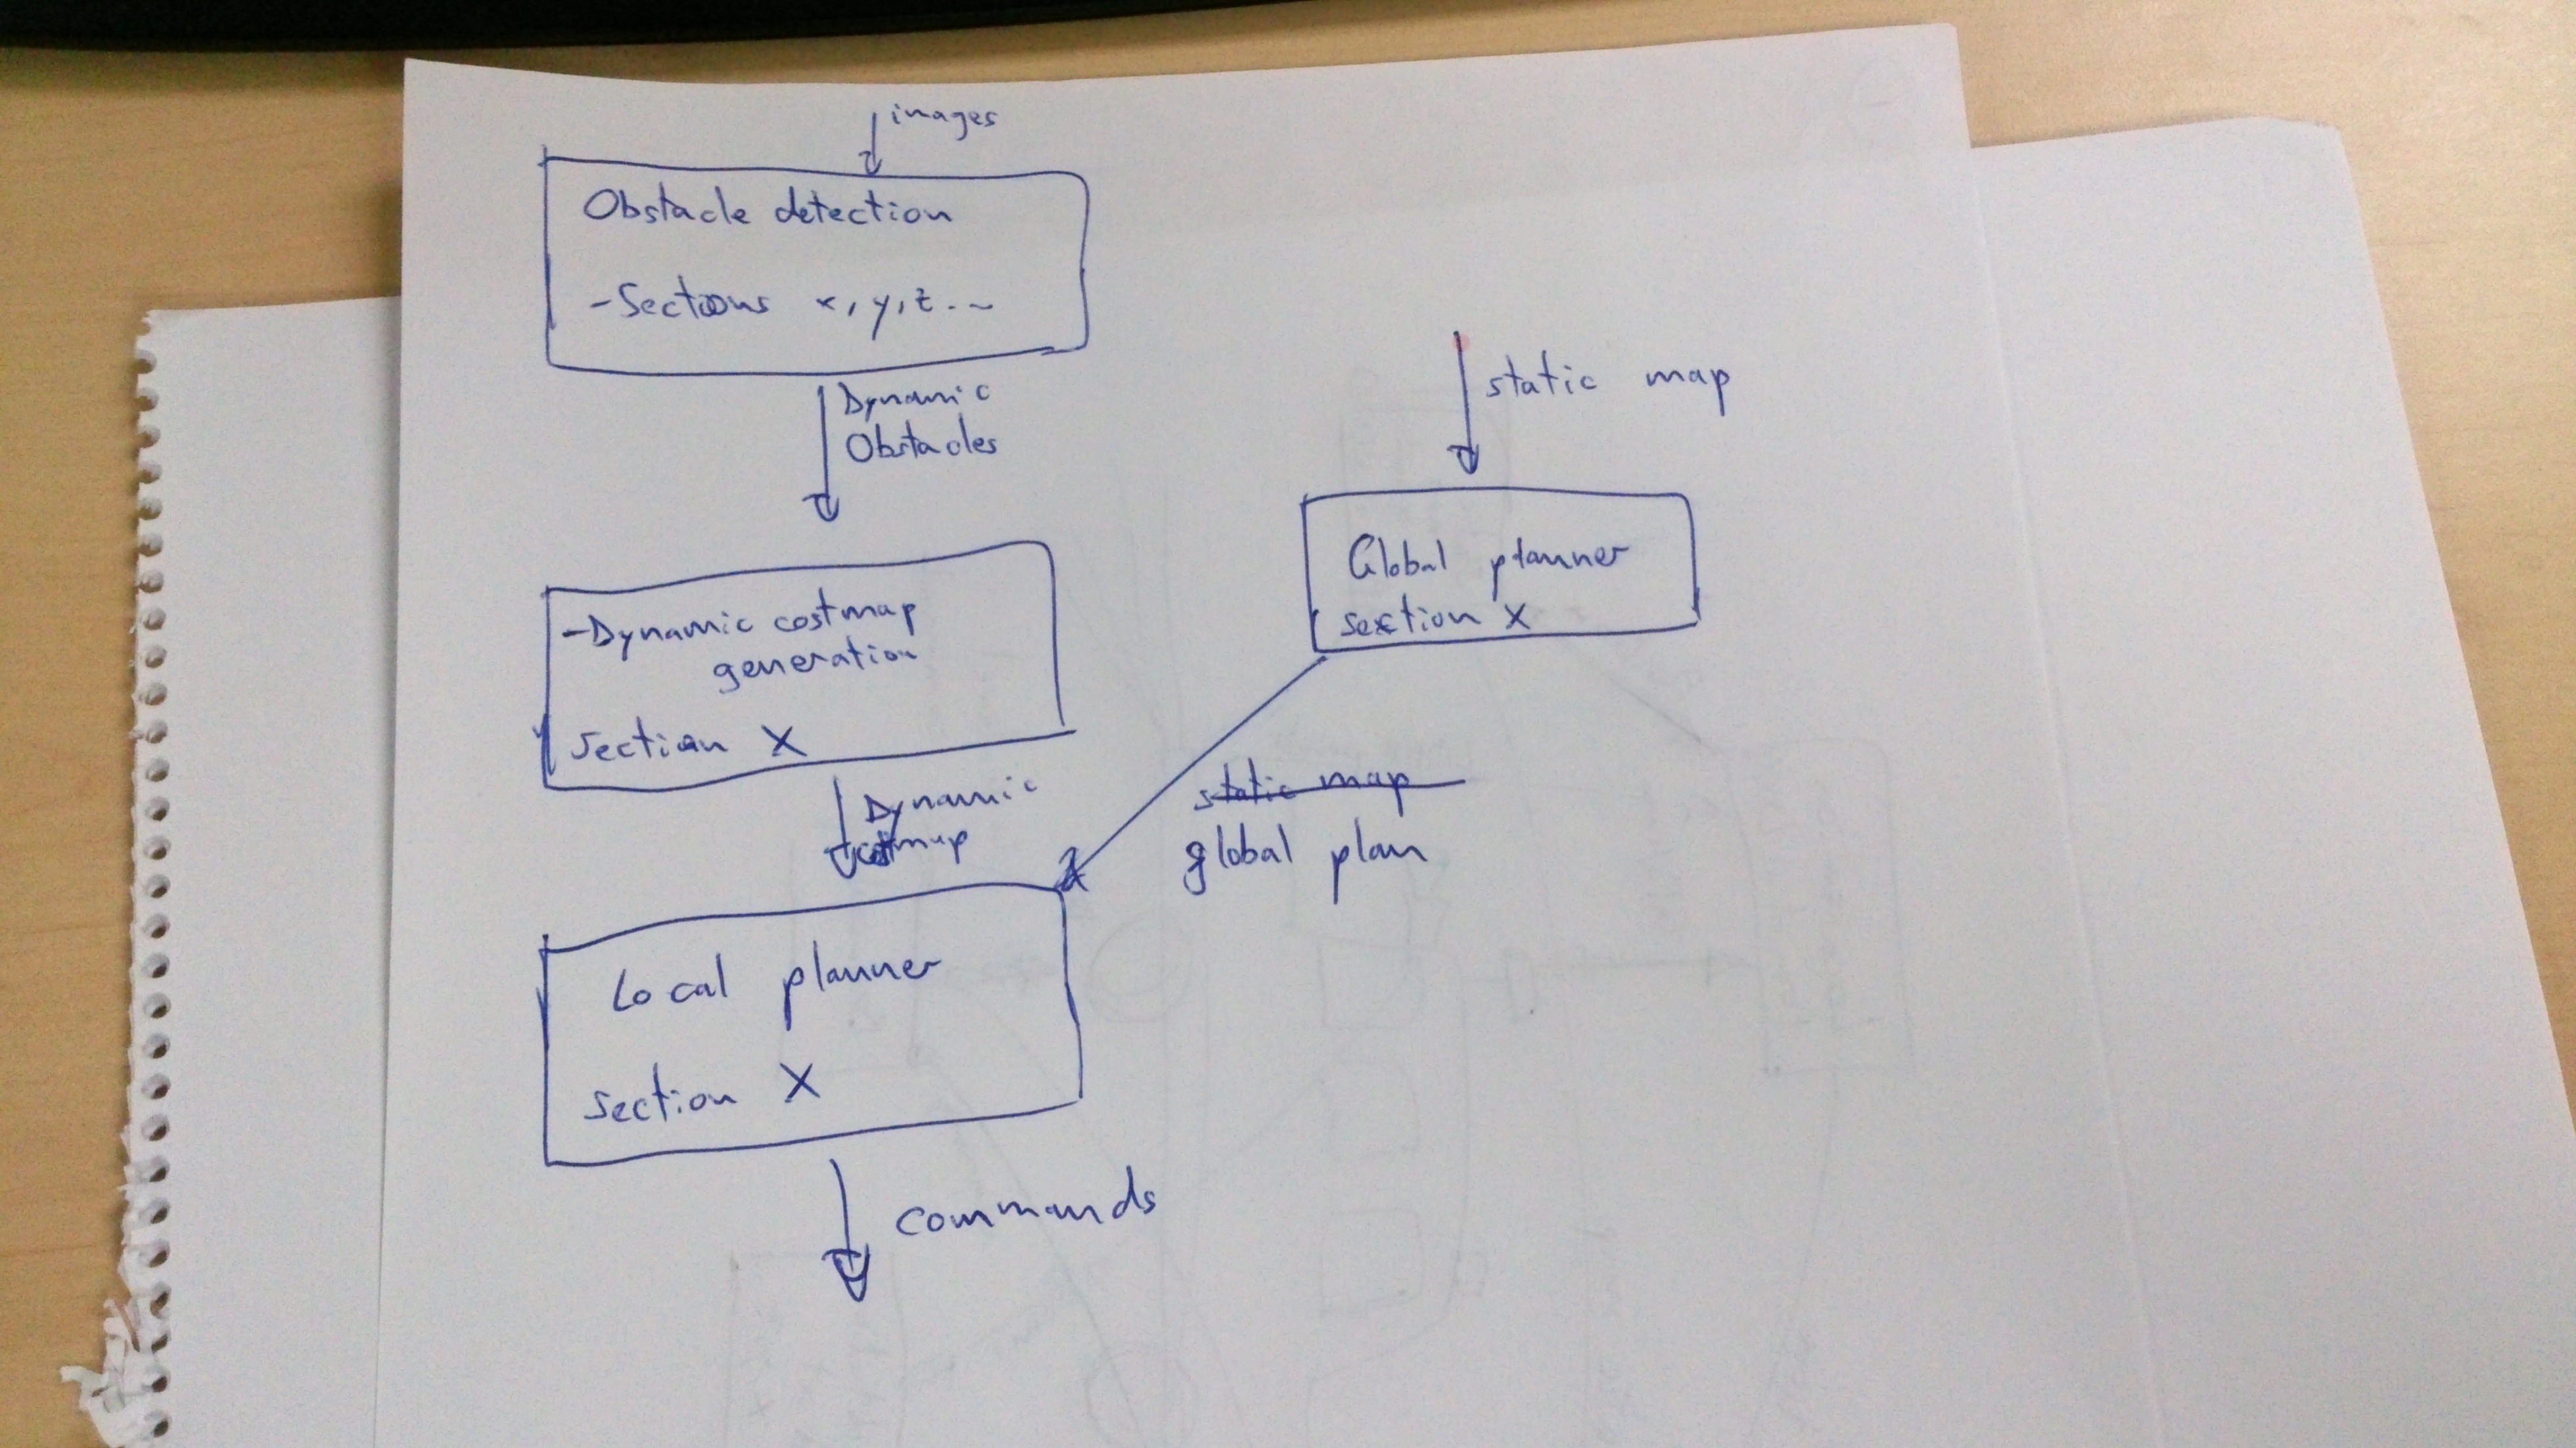
\includegraphics{pipeline}
  \caption{Pipeline of the modules described in this Thesis.}
\end{figure}

From the images captured in real-time, obstacles are located and passed to the module in charge of the generation of the dynamic costmap. At the same time, the static map is used for the generation of a feasible trajectory. Using the current position and vehicle status, the local planner tries to compute the proper commands in order to follow the global plan while trying to avoid the obstacles included in the dynamic costmap.

\section{Previous Work}\label{ch:chapter01_02}

Research on autonomous vehicles is a task being developed for a long time and for which a big effort has been carried on. A proof of that is the extensive literature existing about that topic, in special since the first of the DARPA Challenges (\cite{Buehler2007, Buehler2009}). Since then, the literature related to the topic has increased. Also, the interest on the use of Computer Vision in autonomous vehicles is growing, due to the possibilities that images offer when compared to other sensors, like \acp{LIDAR}.
In 1996, the ARGO project... \todo{Continuar desde aquí, una vez tenga una especie de historia de los vehiculos autonomos, en la intro.}
\todo{TerraMax, VIAC, Braive, Annieway y cualquier otro que pille por el camino.}
As depicted from section \ref{ch:chapter01_01}, the topics described in this thesis are quite diverse, so it is fair to review the state-of-the art of each of these topics separately.

\subsection{Change detection for obstacle localization in images}\label{ch:chapter01_02_01}

\todo{blah blah blah blah blah blah blah blah blah blah blah blah blah blah blah blah blah blah blah blah blah blah blah blah blah blah blah blah blah blah blah blah blah blah blah blah blah blah blah blah blah blah blah blah blah blah blah blah blah blah blah blah blah blah blah blah blah blah blah blah blah blah blah blah blah blah blah blah blah blah blah blah blah blah blah blah blah blah blah blah blah blah blah blah blah blah blah blah blah blah blah blah blah blah blah blah blah blah blah blah blah blah blah blah blah blah blah blah blah blah blah blah blah blah blah blah blah blah blah blah blah blah blah blah blah blah blah blah blah blah blah blah blah blah blah blah blah blah blah blah blah blah blah blah blah blah blah blah blah blah blah blah blah blah blah blah blah blah blah blah blah blah blah blah blah blah blah blah }

\subsection{Non-rigid point set registration for obstacle tracking}\label{ch:chapter01_02_02}

\todo{blah blah blah blah blah blah blah blah blah blah blah blah blah blah blah blah blah blah blah blah blah blah blah blah blah blah blah blah blah blah blah blah blah blah blah blah blah blah blah blah blah blah blah blah blah blah blah blah blah blah blah blah blah blah blah blah blah blah blah blah blah blah blah blah blah blah blah blah blah blah blah blah blah blah blah blah blah blah blah blah blah blah blah blah blah blah blah blah blah blah blah blah blah blah blah blah blah blah blah blah blah blah blah blah blah blah blah blah blah blah blah blah blah blah blah blah blah blah blah blah blah blah blah blah blah blah blah blah blah blah blah blah blah blah blah blah blah blah blah blah blah blah blah blah blah blah blah blah blah blah blah blah blah blah blah blah blah blah blah blah blah blah blah blah blah blah blah blah }

\subsection{Evaluation of stereo 3D reconstruction algorithms}\label{ch:chapter01_02_03}

\todo{blah blah blah blah blah blah blah blah blah blah blah blah blah blah blah blah blah blah blah blah blah blah blah blah blah blah blah blah blah blah blah blah blah blah blah blah blah blah blah blah blah blah blah blah blah blah blah blah blah blah blah blah blah blah blah blah blah blah blah blah blah blah blah blah blah blah blah blah blah blah blah blah blah blah blah blah blah blah blah blah blah blah blah blah blah blah blah blah blah blah blah blah blah blah blah blah blah blah blah blah blah blah blah blah blah blah blah blah blah blah blah blah blah blah blah blah blah blah blah blah blah blah blah blah blah blah blah blah blah blah blah blah blah blah blah blah blah blah blah blah blah blah blah blah blah blah blah blah blah blah blah blah blah blah blah blah blah blah blah blah blah blah blah blah blah blah blah blah }

\subsection{Stixel World}\label{ch:chapter01_02_04}

\todo{blah blah blah blah blah blah blah blah blah blah blah blah blah blah blah blah blah blah blah blah blah blah blah blah blah blah blah blah blah blah blah blah blah blah blah blah blah blah blah blah blah blah blah blah blah blah blah blah blah blah blah blah blah blah blah blah blah blah blah blah blah blah blah blah blah blah blah blah blah blah blah blah blah blah blah blah blah blah blah blah blah blah blah blah blah blah blah blah blah blah blah blah blah blah blah blah blah blah blah blah blah blah blah blah blah blah blah blah blah blah blah blah blah blah blah blah blah blah blah blah blah blah blah blah blah blah blah blah blah blah blah blah blah blah blah blah blah blah blah blah blah blah blah blah blah blah blah blah blah blah blah blah blah blah blah blah blah blah blah blah blah blah blah blah blah blah blah blah }

\subsection{3D object tracking}\label{ch:chapter01_02_05}

By processing the data captured by sensors, it is desired to obtain the position, speed and size of an obstacle. However, usually sensors don't provide this information, so we need to process the information over time and do the tracking of detected obstacles. Many approaches that try to solve this problem, like \cite{danescu2012particle}, assume that obstacles have an standard geometry, and they are modeled as cuboids with associated position, size and speed vectors. This assumption is mostly correct in environments like highways, country roads, and certain urban scenarios, in which almost all the obstacles are cars, trucks or buses which can be simplified as cuboids. Also, these approaches tend to consider a flat ground.
However, this assumption cannot always done, as happens in pedestrian areas, intersections, off-road... In this case, we need to deal with specific shapes, sometimes with concave surfaces. The problem with this kind of obstacles is that methods that assume cuboid-shaped objects tend to wrap the obstacles with a convex shape, which causes an overestimation of their volume (\cite{broggi2013}). Another problem are those objects that are not laying on the ground, as happens with hanged traffic lights, tree crowns, lamps, etc. Usually, they are integrated into an occupancy grid as if they were touching the ground. About the ground plane assumption, in cases like that of an off-road scenario, it is important to estimate the real slope of the road in order to get good results.
Based on how much information they use, we can divide object tracking methods into two subcategories:
\begin{itemize}
 \item \emph{2.5D Solutions:} They do not make use of the complete information provided by 3D points. Instead of that, they tend to use elevation maps composed of uniform size cells. Each cell just stores occupancy and height information. This is the kind of methods that, as described before, usually consider obstacles as being in contact with a flat ground.
 In these methods, tracking is done before the complete reconstruction is done, in an intermediate point based on an specific feature. Based on this intermediate feature, we can distinguishing different kind of approaches:
  \begin{enumerate}
   \item \emph{Use of the 3D point as feature.} An example of this is the so called 6D vision (\cite{franke20056d}), in which the 3D stereo vision extracted information is combined with an efficient implementation of an optical flow in the image space based on a \acf{GPU}. Relevant points are tracked using a Kalman filter.
   \item \emph{Dynamic stixels.} \todo{This approach has been longer discussed in section \ref{ch:chapter01_02_04}.}\comment{Cambiar en caso de que al final no meta los stixels}
   \item \emph{Tracked image features.} As example, check the work by \cite{barth2009estimating}. In this work, obstacles are represented as a rigid 3D point set which are tracked in terms of feature displacements and depth measurements.
   \item \emph{Sensor fusion.} \cite{wu2009collision} reconstruct the objects as cuboids from a stereo point cloud. In this process, position and speed values are improved to a very accurate value by the use of a radar along with stereo.
   \item \emph{Occupancy grids.} This is a very popular choice for tracking. An occupancy grid is a probabilistic map of the driving environment, which encodes the past and present knowledge from sensor data, and which can be updated dynamically when new information is available. These occupancy grids can be cartesian, with rectangular cells, polar, or even a relation between columns in an image an the disparity. An example of this is the method by \cite{danescu2012particle}, which has inspired part of the work described in section \todo { \ref{XXX}}.
   Another advantage of the model based on an occupancy grid is that it makes easier a collaborative update of the grid, which allows the usage of data from several sensors and observers.
  \end{enumerate} 
 \item \emph{3D Solutions:} Usually based on complex grid maps that use complete 3D information. Again, depending on how this grid is represented, we find 
 \begin{enumerate}
   \item \emph{Octree connected cubes.} An example is the work by \cite{wurm2010octomap} or \cite{broggi2013}.
   \item \emph{Adjacent stacks of cells}, as described in \cite{Moravec96robotspatial} 
 \end{enumerate}
\end{itemize}

\subsection{Global planning}\label{ch:chapter01_02_06}

Muchos estudios se han realizado en torno al problema de generacion de rutas globales. Aunque fue inicialmente propuesta para aplicaciones en robotica, ultimamente se ha usado con exito en aplicaciones de automocion.

Podemos dividir los algoritmos de planificacion en... (El resto esta en la libreta, en la parte de estado del arte de planificacion local)


==============================================================
Lo que pongo a continuacion va para la intro de global planning
Los algoritmos de planificacion pueden ser divididos en locales y globales:
Globales:
  La ruta global y los estados del vehiculo quedan determinados por la info proporcionada por un mapa digital y un sistema de localizacion
Locales:
  La ruta local puede ser generada entonces en la etapa de planificacion basada en la ruta global y la info del entorno del vehiculo obtenida por los sensores
  El paper se basa en local path planning que proporciona capacidades de evitacion de obstaculos a un vehiculo autonomo que sigue una ruta global predefinida


\subsection{Local planning}\label{ch:chapter01_02_03}

Con una ruta global calculada y el conocimiento del entorno del vehículo, hace falta enviar al vehículo una serie de comandos que le indiquen cómo seguirla.

En la literatura, muchos métodos se basan en la búsqueda de trayectorias que hagan de intermediarias entre esta ruta global y la ruta local.

Muchos de estos métodos de generación trayectorias se basan en un esquema de optimización discreta (refs. 6, 17-19 coreanos)

Estos métodos calculan un cjto finito de trayectorias basadas en un modelo parametrico, habitualmente funciones polinomiales de un orden determinado. El problema de esto es que a pesar de q el espacio de sol. se reduce y permite una planificacion eficiente, puede introducir suboptimalidad -> Puede llevar a overshoots y/o stationary offsets en curvas

Algunos ejemplos:
(9-annieway) -> Un árbol de trayectorias es muestreado simulando el closed loop system empleando el RRT algorithm
(10-annieway) -> El sistema incorpora varias heurísticas en forma de sampling biases to assert well behaved operation
(17-annieway) El control optimo de un sistema aerodinamico se encuentra dentro de un function space que es spanned by a Garlekin based
Algunos metodos que se basan en la transformacion del espacio de configuraciones mediante el espacio de Frenét:
(Annieway -> Optimal Trajectory Generation for Dynamic Street Scenarios in a Frenét Frame) -> Realiza objetivos a largo plazo como mantenimiento de velocidad, merging, following, stopping por medio de estrategias de ctrol optimo within the Frenét-frame de la calle.
(Stanley: The robot that won the DARPA Grand Challenge) -> Define el offset lateral como la perpendicular a una trayectoria base establecida
  Esta condicion permite al vehiculo circular por la carretera paralelo a la trayectoria base.
  Para seleccionar el path optimo, la funcion de coste penaliza el paso sobre obstaculos y la distancia respecto al centro de la carretera actual
(Coreanos) Tambien genera paths candidatos con endpoints en posiciones fijadas a diferentes offsets respecto al base frame
  Sin embargo, no se basa en el centro de la carretera sino que usa un coste de seguridad para cada path candidato, ya que la estimacion del centro de la carretera puede ser peligroso a la hora de calcular el coste en ciertos escenarios.
  La seguridad de cada path es evaluada cuantitativamente blurring los datos binarios para una colision
  Tb tienen en cuenta como criterios de coste la suavidad y la consitencia del path



\section{Summary}\label{ch:chapter01_03}

In this chapter, we have described a general idea of the work presented in this Thesis. Also, the pipeline of the final developed application is introduced. All this information will be explained in more detail in the following sections, including implementation details together with some results and a discussion of the advantages/disadvantages of the different methods.


%\input{capitulo02}
%\input{capitulo03}
%\acresetall

\graphicspath{{./images/bmps/}{./images/vects/}{./images/}
	      {./images/presentation/bmps/}{./images/presentation/vects/}{./images/presentation/}
	      {./images/chapter00/bmps/}{./images/chapter00/vects/}{./images/chapter00/}}

\begin{frame}{Conclusions}
  \begin{itemize}
   \item Main goal: study of CV based methods for obstacle detection and avoidance applied to the Verdino prototype. 
   \item Four different object detection and tracking approaches.
   \item One method for global planning.
   \item One method for local planning.
   \item A methodology for the automatic evaluation of stereo vision based reconstruction algorithms.
  \end{itemize}
\end{frame}

\begin{frame}{Change Detection for Obstacle Localization in Images}
  \begin{itemize}
   \item Through this approach, we evaluated the influence of the distance and angle difference between the compared images to the quality of the results. 
   \item Conclusions were that the method works properly if distance is below 1\,m and the angle difference is below 10\textdegree. 
   \item We also evaluated the influence of illumination difference between images, concluding that best results were obtained when this difference was below 20\%.
   \item Limitations:
   \begin{enumerate}
    \item If we want to be sure that we fulfill the distance and brightness difference limitations established, we need a highly populated database. 
    \item We can not locate the obstacles detected in real world coordinates since we are working with monocular images.
    \item We can not predict obstacles motion.
   \end{enumerate}
  \end{itemize}
\end{frame}

\begin{frame}{Non-Rigid Contour Tracking}
  \small
  \begin{itemize}
    \only<1> {
    \item With this method, we demonstrated that it is possible to perform contour tracking by using just geometrical information. \item Rhe behavior of four different foreground segmentation methods \citep{lopez2011stochastic, lopez2011foreground, guo2011hierarchical, reddy2012improved} was evaluated, demonstrating that the method presented by \cite{reddy2012improved} is the best for the method requirements.
    \item Same was done for six different non rigid point set registration methods, from which the Coherent Point Drift was the one that gave the best results. 
    }
    \only<2> {
    \item This method was compared with a simple optical flow tracker and a OpenNI Kinect based method. From these tests, we concluded that the behavior is comparable, and usually better than a classical optical flow based contour tracker. Respect to the Kinect based method, our results were reasonable and in certain circumstances outperformed those from the OpenNI method.
    \item The main limitation is that we are tied to the use of static cameras.
    }
  \end{itemize}
\end{frame}

\begin{frame}{Evaluation of Stereo 3D Reconstruction Algorithms}
  \small
  \begin{itemize}
  \only<1> {
    \item Choosing an specific dense reconstruction algorithm or another is, \emph{a priori}, a difficult task. In this thesis, an automatized framework for the evaluation of dense reconstruction algorithms was developed.
    \item This framework allows testing algorithms from long sequences of images, at different weather and illumination conditions. This solves the problem existing for other previous evaluations in which testing images are taken in laboratories, under controlled conditions; or are based on too short sequences, where ground truth is edited by hand.
    \item We demonstrated that it is possible to do an evaluation on the performance of the methods without the need of a LIDAR-based ground truth (which, despite of the great reliability of the statistics obtained with it, is quite expensive in terms of the required equipment and the time needed for post-processing the captured data). 
    }
    \only<2> {
    \item The use of a prior on the vehicle movement was successfully exploited to identify a portion of the wrongly reconstructed points, making it suitable for evaluation of big data-sets, thus covering a broad range of environmental conditions. 
    \item In the other hand, the use of a third camera for evaluation looks feasible, but in practice obtained results were not very discriminative.
    \item With these evaluation strategies, we concluded that the use of filtering strategies reduces the number of wrong pixels and enhances the accuracy of the results. 
    }
  \end{itemize}
\end{frame}

\begin{frame}{Stixel World}
  \small
  \begin{itemize}
    \item We successfully developed a method for obstacle detection and tracking based on the stixel world described in \cite{badino2009stixel}. 
    \item With this work, we demonstrated that the use of a two-level tracking outperforms existing stixel based tracking methods. \item Also, we discovered that the use of the Hellinger distance instead of the SAD improves tracking results, and we saw that the effect of factor $\alpha_{height}$ on tracking results is negligible. 
    \item We showed that if speed is preferred over accuracy, object based tracking is possible, in which objects are obtained through a simple clustering method and then are tracked by using the illumination information between the obstacles.
  \end{itemize}
\end{frame}

\begin{frame}{Particle Filter based Object Tracking}
  \small
  \begin{itemize}
  \only<1> {
    \item We developed a tracking method able to receive a point cloud as input and detect objects and their movement direction and speed, based just on their position in real world coordinates and a particle filter. 
    \item Although we centered this work on dense stereo reconstruction based point clouds, it is also able to work with point clouds provided by other sensors, like for example LIDARs, as we are not using color information. 
    \item The use of a particle filter based approach allows avoiding complex calculations associated to the computation of probabilities, and the use of a voxel grid allows working in three dimensions without increasing the complexity. It also allows a more specific knowledge of obstacles, better than other representations of obstacles, like cuboids.
    }
    \only<2> {
    \item Our method is compared with the method of \cite{danescu2012particle}, concluding that, despite the obtained recall in the detection is almost similar (being slightly better the values obtained by our implementation), the precision obtained with our method outperforms theirs. 
    \item We wanted to know which of the available stereoscopic 3D reconstruction methods is the most suitable to be used as input, concluding that ELAS is the best choice from all the available methods.
    \item Some tests were also done in order to ensure that the localization method described in \cite{geiger2011stereoscan} is a valid substitute of the localization provided by mechanical odometry, concluding that both of them are equally reliable.
    }
  \end{itemize}
\end{frame}

\begin{frame}{Global Planning}
  \small
  \begin{itemize}
    \item We developed an innovative strategy for generating trajectories based on a Multiclass Support Vector Machine, in which each obstacle is a class, and the decision borders are the possible paths. 
    \item Advantages of using this method as a base is that we can generate continuous non-linear border lines that allow the creation of smooth, short and safe paths. The use of the GPU reduces the required computational time.
    \item This method was compared to other state of the art SVM planners, showing that our method outperforms all of them in terms of average distance to obstacles, smoothness and length of the computed paths. It was also compared to other classical methods, like \emph{Voronoi}, obtaining also better results with our approach.
  \end{itemize}
\end{frame}

\begin{frame}{Local Planning}
  \small
  \begin{itemize}
    \item We developed a method that based on the Frenét space, is able to generate smooth paths that allow, at the same time, following the computed trajectory and avoiding obstacles in the way. 
    \item Generation of tentative paths is simplified as speed is out of the model for the tracks generation, so the problem is reduced to the computation of a set of parameters that define a third order polynomial. We also use different lateral offsets with respect to the global plan, so avoidance of obstacles is considered. Then, the use of a cost function allows selecting the best path.
    \item In our tests, we demonstrated that the described method is able to accurately follow a given trajectory. We also saw the effect produced by each cost factor independently, and that their integration conducts to a safe and efficient behavior in the trajectory following procedure.
  \end{itemize}
\end{frame}

\begin{frame}{Putting all together}
  \footnotesize
  \begin{itemize}
    \item Local planner was integrated with the stixel and the particle filter based methods. As the implemented costmap is reduced to a bidimensional grid in which no temporal information can be included, we were just able to integrate the top-view projection of the detected obstacles.
    \item However, integration of obstacles was satisfactory, allowing in our simulations to perform a safe navigation between the obstacles using both KITTI \citep{geiger2013vision} and Bahnhoff \citep{ess2009robust} datasets. 
    \item Using the stixel or the particle filter based approach, it is a decision that must be taken and that depends on the suitability of the environment to the characteristics of each method, as well as on the requirements of each application. \item Particle filter based method is more generalist, as we do not take special assumptions in this approach; however, if assumptions made for the stixel based approach are fulfilled, this method is much faster, specially if we do not need to perform an accurate tracking (which would allow us to use just the object based tracking method).
  \end{itemize}
\end{frame}

\begin{frame}{Future work}
  \footnotesize
  \begin{itemize}
    \only<1> {
    \tiny
    \item Change Detection for Obstacle Localization in Images
    \begin{itemize}
      \tiny
      \item Using other methods for the matching of features between images is possible. In fact, we have done some tests in which we used the GPU for the computation and matching of SURF features (\cite{bay2008speeded}), in which times obtained were acceptable for this approach.
%       \item We could also implement a shadow detector, in order to reduce the similarity on the illumination requirements.
      \item Some of the techniques used in the image database based method could be also used for other related tasks like the improvement of some of the existing change detection methods for aligned video sequences, as for example those presented in \cite{diego2011video, evangelidis2011slice, evangelidis2011efficient}.
    \end{itemize}
    \tiny
    \item Non-Rigid Contour Tracking
    \begin{itemize}
      \tiny
      \item Output obtained for the non rigid contour tracking method could be used for many applications, not just related to ADAS, but also to motion analysis in videos or HMI systems.
      \item We would like to go beyond the use of static bidimensional image sequences, and extend the contour tracking method to be used with 3D information. A way to do that could be the segmentation of a disparity map, in which the contours used would be the borders of the segmented regions. These could be easily transformed to real world coordinates, once the tracking step is finished.
      \item Another way to do that would be through the addition of new dimensions to the points used in the non-rigid point set registration step. Despite the Coherent Point Drift algorithm allows doing that, it would require to optimize the current implementation of this method. This will also allow including color information easily. We started a CUDA based implementation of this method, with promising results.
      \item We would like to extend the trilateration based motion detector method used in the results section for the evaluation, so it is used for the analysis of an object motion. This would require to generate an initial model of the tracked object, but the analysis of its movement could be done through our method.
    \end{itemize}
    }
    \only<2> {
    \item Evaluation of Stereo 3D Reconstruction Algorithms
    \begin{itemize}
      \item About the evaluation of dense reconstruction methods, the use of a third camera for the comparison with a reconstructed virtual image was promising, but results were not as good as expected. In the future, we could use different metrics to measure the similarity between the control camera and virtual images. 
      \item More experiments could be performed, including sequences with different weather conditions.
    \end{itemize}
    }
    \only<3> {
    \tiny
    \item Stixel World
    \begin{itemize}
      \tiny
      \item We also want to try new methods for stixel computation. A possibility could be using polar rectification for the combination of tracking and reconstruction in a single process. 
      \item We could use the tracking output as a clue for the clustering process, in which we just consider the stixels for which a correspondence was found.
    \end{itemize}
    \item Particle Filter based Object Tracking
    \begin{itemize}
      \tiny
      \item The particle filter could be extended so color information is also used. This would prevent the use of sensors different from stereo cameras, but we could think on an schema in which the information provided by several sensors is combined, being a stereo pair one of them.
      \item We could track the particles along frames, which would improve results and also would increment the knowledge we have about obstacles.
      \item Taking advantage of the big amount of operations that are performed independently for each voxel, we think that a parallel implementation of the method is easy to achieve and will reduce drastically the required time.
    \end{itemize}
    }
    \only<4> {
    \item Global Planning
    \begin{itemize}
      \item Regarding to path planning methods, there also some work that could be done. For example, new clustering strategies could be applied for the global planner, and the use of MSVM could be combined with other classical approaches.
    \end{itemize}
    \item Local Planning
    \begin{itemize}
      \item New cost of long-term control strategies could be applied for the generation and selection of the candidate paths in the local planner, as done in \cite{werling2010optimal}.
      \item In the local planner, the final selection of applied steering angle and speed could be improved. Some approaches we have considered are based on the use of a predictive controller.
    \end{itemize}
    }
    \only<5> {
    \item Finally, we would like to improve the costmap computation scheme, so full-3D information (in the form of voxels or other similar approach, for instance) will allow making use of more accurate information about the obstacles. In special, we would like to include temporal information, so we will be able to perform a more intelligent navigation, in which we consider both the present and the future of the environment for a safe and enjoyable trip.
    }
  \end{itemize}
\end{frame}

{
\setbeamertemplate{background canvas}{\hskip-0.2cm\begin{tikzpicture}\node[opacity=1.0]{\includegraphics[height=\paperheight]{background}};\end{tikzpicture}}
\begin{frame}[plain]{Questions?}
%   \begin{overlayarea}{2\textwidth}{\textheight}
%     \vskip-0.7cm \hskip-1cm
%     \begin{center}
%       \includegraphics[width=\textwidth]{background}
%     \end{center}
%   \end{overlayarea}
%     
\includegraphics[width=\textwidth]{thankyou}

\end{frame}
}


\appendix
%%
%% apendiceA.tex - Memoria de la tesis
%%
%%   Copyright 2009-2010 Jesús Torres <jmtorres@ull.es>
%%
%% Esta obra está bajo licencia Creative Commons Reconocimiento 3.0 Unported
%%
\chapter{Apéndice A}
Lorem ipsum dolor sit amet, consectetur adipiscing elit. Vestibulum faucibus
sollicitudin facilisis. Donec sollicitudin augue eu lectus gravida mollis.
Nunc lacinia imperdiet posuere. Curabitur augue nulla, placerat sit amet
pellentesque a, venenatis id ante. Ut eget neque eros, sit amet ornare risus.
Quisque quis blandit tortor. Donec nunc justo, consectetur ac tempor eget,
dignissim ut arcu. Nam eu justo vel est imperdiet dignissim. Phasellus
vulputate augue nec est tincidunt fermentum. Sed hendrerit nisl sed turpis
blandit vestibulum. Vestibulum vitae lectus ac ligula varius iaculis. Maecenas
vitae lorem arcu, nec convallis leo. Nulla cursus, odio sit amet semper
hendrerit, odio magna dignissim massa, ut mattis justo felis at ante. Class
aptent taciti sociosqu ad litora torquent per conubia nostra, per inceptos
himenaeos.

\section{Sección 1 del apéndice A}\label{sec:apendice}
\lstCppMakeShortInline|
Nunc tincidunt fringilla dictum. In ac dolor et nibh viverra sodales a vitae
purus. Curabitur ultricies bibendum dolor eget lacinia. Duis fermentum neque
sit amet purus tempus in porta mauris posuere. Sed sit amet nulla odio. Nam
sit amet fermentum lorem. Mauris accumsan suscipit lorem. Suspendisse sed
nulla mi, id viverra tellus. Ut tristique egestas eros, ut molestie risus
aliquam nec. In aliquet, mi sit amet |'fringilla'| cursus, nisl velit
tincidunt lacus, in euismod lorem erat sit amet urna. Quisque ultrices luctus
odio sollicitudin |'malesuada'|.

\lstDeleteShortInline|

%\input{apendiceB}

\backmatter
\bibliography{references}

\end{document}
